\def\mytitle{PYTHON PROGRAMMING ON MATRICES}
\def\myauthor{V.Meghana}
\def\contact{r170237@rguktrkv.ac.in}
\def\mymodule{Future Wireless Communication (FWC)}


\documentclass[10pt, a4paper]{article}
\usepackage[a4paper,outer=1.5cm,inner=1.5cm,top=1.75cm,bottom=1.5cm]{geometry}

\twocolumn
\usepackage{graphicx}
\usepackage{karnaugh-map}
\usepackage{tabularx}
\usepackage{hyperref}
\usepackage[utf8]{inputenc}
\usepackage{amsmath}
\usepackage{physics}
\usepackage{amssymb}
\usepackage{watermark}
\renewcommand*\familydefault{\sfdefault}
\usepackage{lipsum}
\usepackage{xcolor}
\usepackage{listings}
\let\vec\mathbf
\lstset{
frame=single, 
breaklines=true,
columns=fullflexible
}

\begin{document}
\title{\mytitle}
\author{\myauthor\hspace{1em}\\\contact\\FWC22045\hspace{6.5em}IITH\hspace{0.5em}\mymodule\hspace{6em}Matrix:Lines}

%\{ Wireless Communication (FWC)}
\date{}
\maketitle


  \section{Problem}
Three distinct points A, B and C are given in the 2-dimensional coordinates plane such that the ratio of the distance of any one of them from the point (1, 0) to the distance from the point (-1, 0) is equal to 1:3 . Then the circumcentre of the triangle ABC is at the point:

\section{Solution}
\begin{center}

%\boldmath

$$\vec{P}=\begin{pmatrix} 1\\ 0\ \end{pmatrix} ...(1)$$
$$\vec{Q}=\begin{pmatrix} -1\\ 0\ \end{pmatrix} ...(2)$$
%\unboldmath
\end{center}

\textbf{Given that:}
\\
Distance between any vertex of a triangle to points P and Q is
\\
\begin{center}
%\boldmath
$\frac{\norm{\vec{A-P}}}{\norm{\vec{A-Q}}}$=$\frac{\norm{\vec{B-P}}}{\norm{\vec{B-Q}}}$=$\frac{\norm{\vec{C-P}}}{\norm{\vec{C-Q}}}$=$\frac{1}{3} ...(3)$
%\unboldmath
\end{center}

\textbf{Circumcentre:} \\

The circumcenter of a triangle is defined as the point where the perpendicular bisectors of the sides of that particular triangle intersect.
\\
Circumcentre interms of vector is
\\
\begin{center}
%\boldmath
$\norm{\vec{A-O}}$=$\norm{\vec{B-O}}$=$\norm{\vec{C-O}}=r...(4)$
\\
%\unboldmath
\end{center}
\begin{center}
%\boldmath
$\frac{\norm{\vec{A-P}}^2}{\norm{\vec{A-Q}}^2}$=$\frac{\norm{\vec{B-P}}^2}{\norm{\vec{B-Q}}^2}$=$\frac{\norm{\vec{C-P}}^2}{\norm{\vec{C-Q}}^2}$=$\frac{1^2}{3^2}...(5)$\\
$$9(A-P)^T.(A-P)=(A-Q)^T.(A-Q) ...(6)$$\\
$$9A^T.A-18P^T.A+\norm{\vec{P}}^2=A^T.A-2Q^T.A+\norm{\vec{Q}}^2 ...(7)$$\\
$$8A^T.A-2(9P-Q)^T.A+\norm{\vec{P}}^2-\norm{\vec{Q}}^2=0 ...(8)$$\\
$$8.\norm{\vec{A}}^2+2(Q-9P)^T.A+\norm{\vec{P}}^2-\norm{\vec{Q}}^2=0...(9)$$\\
Similarly, we can do this for B and C\\
$$8.\norm{\vec{B}}^2+2(Q-9P)^T.B+\norm{\vec{P}}^2-\norm{\vec{Q}}^2=0...(10)$$\\
$$8.\norm{\vec{C}}^2+2(Q-9P)^T.C+\norm{\vec{P}}^2-\norm{\vec{Q}}^2=0...(11)$$\\
By squarring the circumcentre equation on both sides,we get\\
$$\norm{\vec{A-O}^2}=\norm{\vec{B-O}^2}=\norm{\vec{C-O}^2}=r^2...(12)$$\\
By expanding the terms,
$$\norm{\vec{A}}^2-2(A)^T.O+\norm{\vec{O}}^2=r^2...(13)$$\\
$$\norm{\vec{B}}^2-2(B)^T.O+\norm{\vec{O}}^2=r^2...(14)$$
$$\norm{\vec{C}}^2-2(C)^T.O+\norm{\vec{O}}^2=r^2...(15)$$\\
Subtract the eqns (13),(14) and (14),(15) then we get\\
$$O^T.(A-B)=\frac{\norm{\vec{A}}^2-\norm{\vec{B}}^2}{2}...(16)$$\\
$$O^T.(B-C)=\frac{\norm{\vec{B}}^2-\norm{\vec{C}}^2}{2}...(17)$$\\
Subtract the eqns (9),(10) and (10),(11) then we get\\
$$\frac{1}{8}.[(Q-9P)^T.(A-B)]=\frac{\norm{\vec{A}}^2-\norm{\vec{B}}^2}{2}...(18)$$
$$\frac{1}{8}.[(Q-9P)^T.(B-C)]=\frac{\norm{\vec{B}}^2-\norm{\vec{C}}^2}{2}...(19)$$\\
By comparing equations (16),(18) and (17),(19) we get\\
$$O=\frac{1}{8}.(9P-Q) ...(20)$$\\
By substituting the P and Q values we get the Circumcentre,\\
$$\vec{O}=\begin{pmatrix} \frac{5}{4}\\ 0\ \end{pmatrix} $$

\end{center}
%\unboldmath
 
\section{Construction}
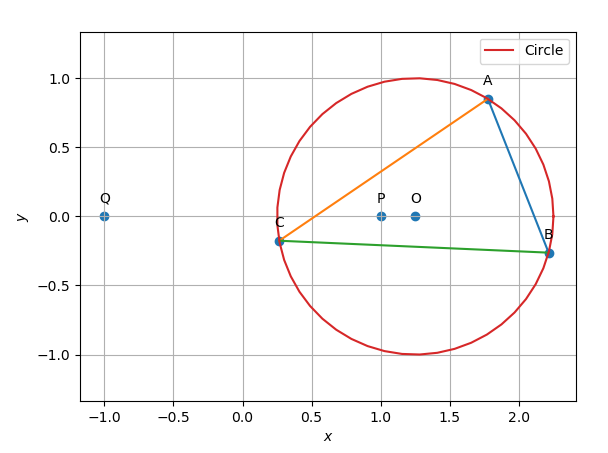
\includegraphics[scale=0.5]{circum.png} 
    
\section{Execution}
*Verify the above proofs in the following code.\\
\begin{lstlisting}
https://github.com/pavan170850/Fwciith2022/blob/main/Matrix_Lines/codes/para.py
\end{lstlisting}
	

\bibliographystyle{ieeetr}
\end{document}